% ==========================================
% BAB IV DESAIN KONSEP SOLUSI
% ==========================================
\chapter{DESAIN KONSEP SOLUSI}
\label{chap:desain-konsep-solusi}

Bab ini menjelaskan desain konsep solusi implementasi AI dalam perencanaan anggaran pada usaha kecil dan menengah (UKM). Bab ini akan meliputi \textit{use case, flowchart}, dan arsitektur sistem.

% ------------------------------------------------
\section{Aktor dan Use Case}
% ------------------------------------------------

Untuk menegaskan ruang lingkup sistem, aktor yang terlibat, dan menentukan batas interaksi pengguna dengan sistem, diagram berikut memetakan tiga fungsi utama yang akan didukung yaitu rekomendasi anggaran proyek, validasi pengajuan anggaran, serta analisis kelayakan produk/usaha baru.

\begin{figure}[h] % pilihan opsi yang disarankan: t = top, b = bottom, h = here
	\centering
  \captionsetup{justification=centering}
    	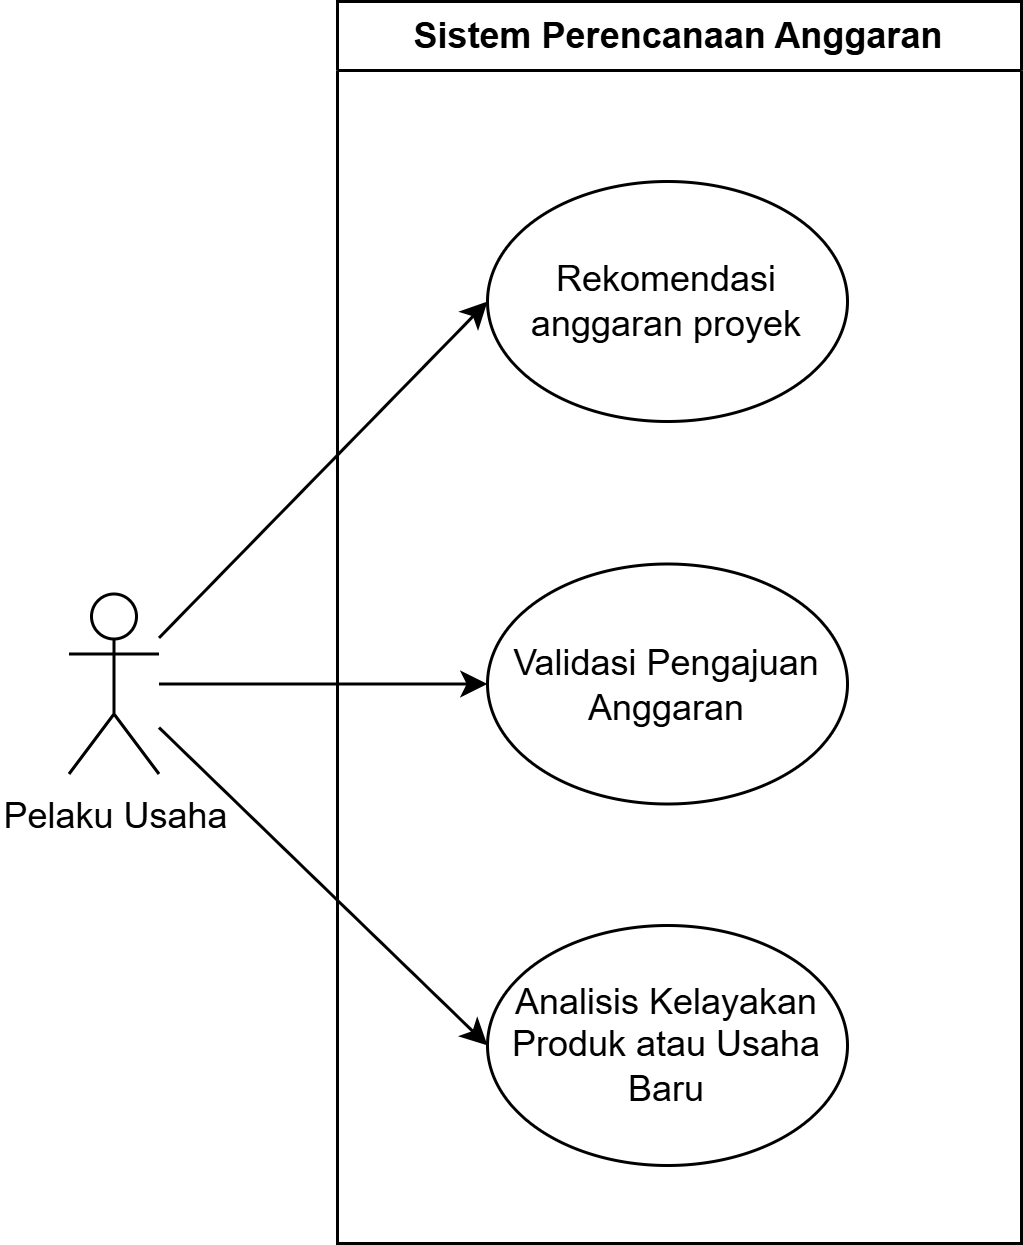
\includegraphics[width=0.5\textwidth]{image/Use Case.png}
	\caption{\textit{Use Case} Sistem}
	\label{gambar:Use Case}
\end{figure}

Agar elemen pada diagram tersebut mudah dilacak, ringkasan tiap \textit{use case} disajikan pada tabel berikut. Tabel ini merangkum tujuan, keluaran yang diharapkan, dan akan menjadi acuan saat menyusun alur proses (To-Be) pada bagian selanjutnya.

\begin{longtable}{|p{2cm}|p{5cm}|p{7.5cm}|}
\caption{Daftar \textit{Use Case} Sistem}
\label{tbl:use-case} \\
\hline
\textbf{Kode} & \textbf{\textit{Use Case}} & \textbf{Deskripsi} \\
\hline
\endfirsthead

\hline
\textbf{Kode} & \textbf{\textit{Use Case}} & \textbf{Deskripsi} \\
\hline
\endhead

\hline
\multicolumn{3}{r}{\textit{Bersambung ke halaman berikutnya}} \\
\endfoot

\hline
\endlastfoot

UC-01 & Rekomendasi Anggaran Proyek &
Pengguna memperoleh rekomendasi alokasi anggaran proyek yang lebih tepat beserta alasan dan referensi dokumen pendukung. \\ \hline

UC-02 & Validasi Pengajuan Anggaran &
Pengguna mendapatkan penilaian kelayakan suatu pengajuan (mis.\ peningkatan perangkat atau belanja tertentu) berdasarkan bukti, aturan, dan analisis yang relevan. \\ \hline

UC-03 & Analisis Kelayakan Produk/Usaha Baru &
Pengguna mendapatkan peenilaian kelayakan memasuki produk atau pasar baru dengan mempertimbangkan kondisi internal, referensi pasar, risiko, dan prasyarat eksekusi. \\ \hline

\end{longtable}

% ------------------------------------------------
\section{Alur Utama Sistem (To-Be)}
% ------------------------------------------------

Berdasarkan tiga use case di atas, alur To-Be berikut menggambarkan langkah end-to-end dari input pengguna hingga keluaran sistem. Langkah bernuansa terotomasi merepresentasikan proses yang dijalankan mesin (orkestrasi, \textit{retrieval, reasoning}), sedangkan langkah lainnya menunjukkan keputusan/aktivitas organisasi yang tetap berada pada kendali pengguna.

\begin{figure}[h] % pilihan opsi yang disarankan: t = top, b = bottom, h = here
	\centering
  \captionsetup{justification=centering}
    	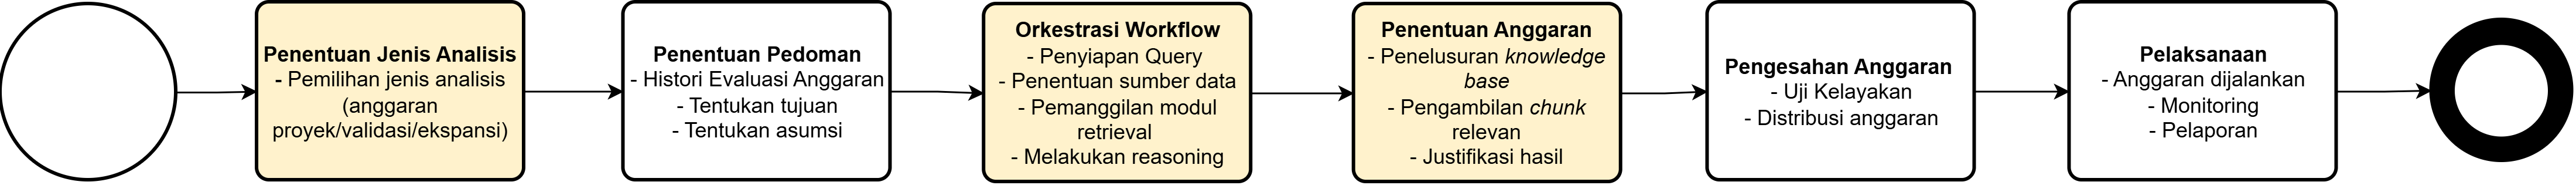
\includegraphics[width=1\textwidth]{image/To Be Flowchart.png}
	\caption{Alur utama sistem (To-Be)}
	\label{gambar:flow-to-be}
\end{figure}	

Proses dimulai dari penentuan jenis analisis oleh pengguna. Hal ini berupa pemilihan untuk ingin melakukan anggaran proyek, validasi pengajuan, atau ekspansi usaha. Pilihan ini akan menentukan parameter input yang dibutuhkan serta jalur proses selanjutnya. Setelah itu, pengguna menetapkan pedoman analisis berupa tujuan periode, asumsi utama (misalnya permintaan, biaya, atau kapasitas), dan bila ada, hasil evaluasi anggaran sebelumnya sebagai konteks bisnis. Sistem kemudian melakukan orkestrasi \textit{workflow}, yaitu menyusun kueri dari input tersebut, memilih sumber data (dokumen pedoman, histori, atau referensi pasar), lalu memanggil modul \textit{retrieval} dan meneruskan konteksnya ke modul reasoning. Pada tahap penentuan anggaran, mesin melakukan RAG dengan menelusuri \textit{knowledge base}, mengambil chunk paling relevan, dan menyusun rekomendasi berikut justifikasinya berdasarkan mode analisis yang dipilih. Selanjutnya masuk ke pengesahan anggaran, di mana hasil sistem diuji kelayakannya (misalnya melalui batas biaya atau ambang ROI) sebelum didistribusikan sebagai acuan pelaksanaan. Terakhir, pada tahap pelaksanaan, anggaran dijalankan dan dilakukan monitoring serta pelaporan realisasi, lalu data tersebut kembali menjadi artefak dan \textit{evidence} untuk siklus evaluasi berikutnya.

% ------------------------------------------------
\section{Arsitektur Sistem Berlapis}
% ------------------------------------------------

\begin{figure}[h] % pilihan opsi yang disarankan: t = top, b = bottom, h = here
	\centering
  \captionsetup{justification=centering}
    	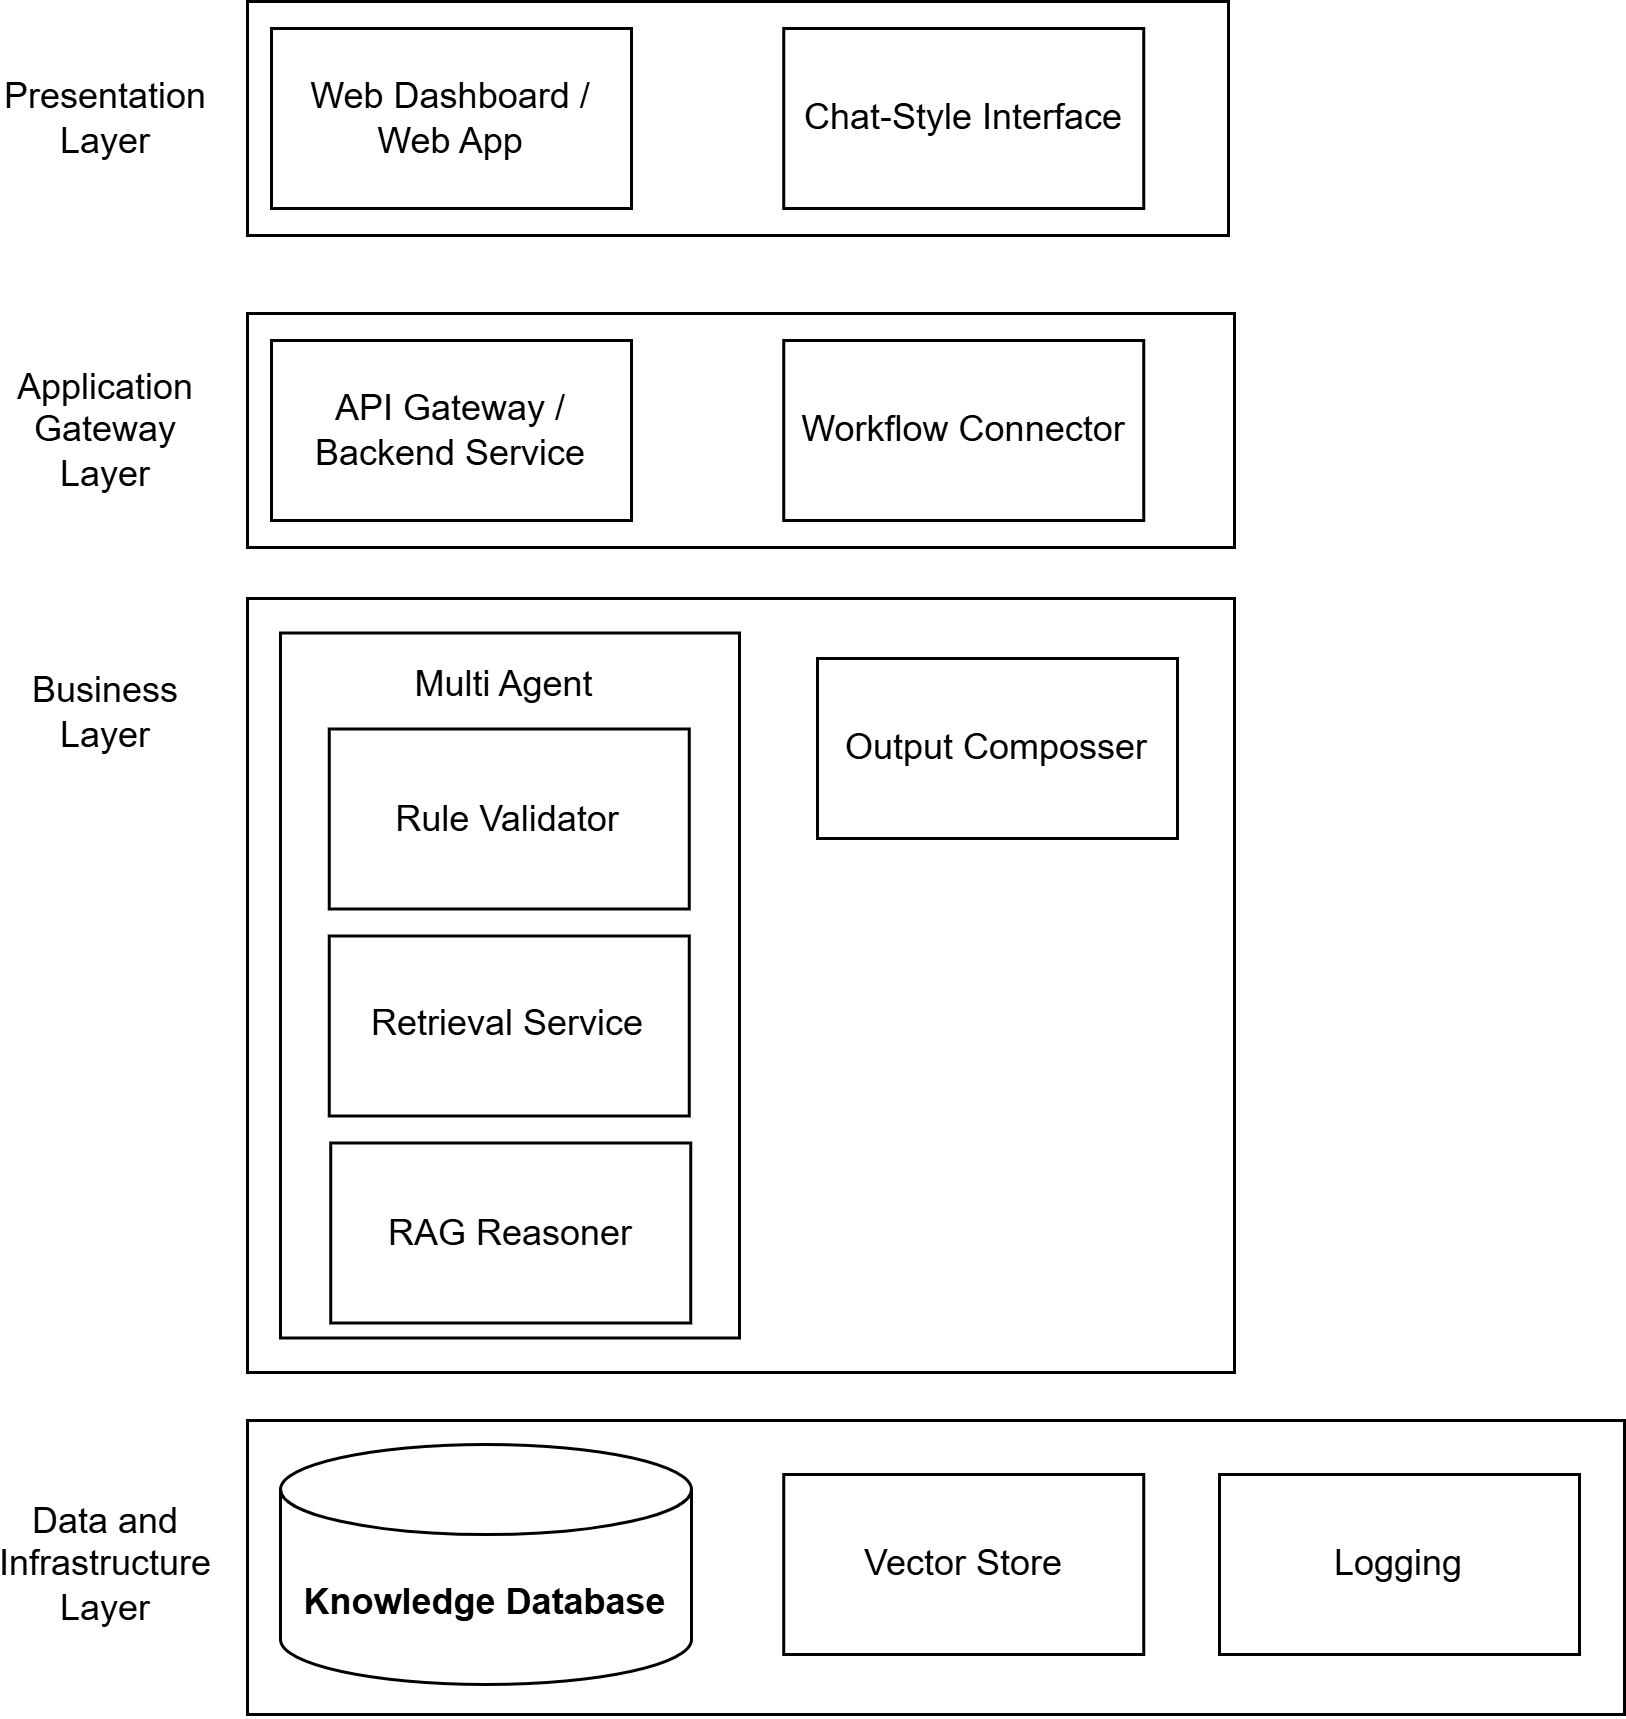
\includegraphics[width=0.9\textwidth]{image/Architecture system.png}
	\caption{Arsitektur sistem berlapis}
	\label{gambar:architecture}
\end{figure}

Diagram arsitektur sistem Gambar \ref{gambar:architecture} menggambarkan seluruh komponen sistem bekerja. Masing-masing lapisan memiliki fungsi yang saling melengkapi.

\begin{enumerate} 
	\item \textit{Presentation Layer}\\ 
	Pada lapisan pengguna berinteraksi melalui \textit{Web Dashboard dan Chat-Style Interface} untuk memilih mode analisis, mengisi input seperti periode, asumsi permintaan atau biaya, mengunggah dokumen, serta melihat hasil evaluasi berupa ringkasan rekomendasi, alasan, risiko, referensi, dan status proses. 
	\item \textit{Application Gateaway Layer}\\ 
	Lapisan ini berperan sebagai pintu masuk seluruh request dari antarmuka. Di layer ini dilakukan autentikasi, validasi dan normalisasi input, penyusunan kueri dan payload, serta orkestrasi pipeline melalui \textit{Workflow Connector}. 
	\item \textit{Business Layer}\\ 
	Lapisan terdiri dari \textit{Multi Agent dan Output Composer. Multi Agent} mencakup \textit{Rule Validator} untuk memeriksa batas biaya dan ambang ROI, \textit{Retrieval Service} untuk membangun embedding dan menemukan dokumen relevan, serta RAG Reasoner yang menggabungkan input dan konteks untuk menghasilkan rekomendasi yang dapat dijelaskan. \textit{Output Composer} kemudian menyusun hasil akhir ke dalam bentuk terstruktur seperti Rangkuman, Alasan, Risiko, Rekomendasi, dan Referensi. 
	\item \textit{Data and Infrastructure Layer}\\ 
	Lapisan ini yang memuat \textit{Knowledge Database} berisi dokumen pedoman, histori, dan referensi pasar beserta metadata. Lalu ada \textit{Vector Store} untuk penyimpanan \textit{embedding} dan operasi \textit{similarity search}. Selanjutnya terdapat \textit{Logging} yang mencatat jejak input, dokumen yang digunakan, dan versi komponen sebagai dasar monitoring dan audit. Secara keseluruhan, pemetaan prosesnya adalah: penentuan jenis analisis dan pedoman terjadi di \textit{Presentation Layer}, orkestrasi \textit{workflow di Application Gateway}, penelusuran \textit{knowledge base} dan penyusunan rekomendasi di \textit{Business dan Data Layer}. Pengesahan dan pelaksanaan terjadi di \textit{Presentation Layer} dan proses organisasi di luar sistem. 
\end{enumerate}

% \section{Perbandingan Sistem Tradisional dan Sistem Berbasis AI}
% Subbab ini menguraikan perbandingan antara pendekatan tradisional dan pendekatan berbasis AI dalam dua aspek utama, yaitu akurasi perencanaan anggaran dan akurasi \textit{forecasting}.


% \subsection{Akurasi Perencanaan Anggaran}
% Pendekatan tradisional umumnya bersifat statis dan tidak mampu melakukan penyesuaian otomatis ketika terdapat perubahan dalam proyeksi pendapatan atau kondisi operasional. Penelitian tentang penggunaan AI dalam aktivitas perencanaan menunjukkan bahwa AI dapat meningkatkan efektivitas pengelolaan anggaran dengan mengidentifikasi pola pengeluaran yang tidak efisien dan memberikan saran alokasi yang lebih tepat \autocite{chen2021}.
% \subsection{Akurasi \textit{Forecasting}}


% Ilustrasikan desain konsep solusi dalam bentuk model konseptual dan penjelasan secara ringkas, 
% beserta perbedaannya dengan sistem saat ini. Ilustrasi harus dapat dibandingkan (\textit{before} and \textit{after}). 
% Karena masih berupa proposal, bab ini hanya berisi gambar desain konsep solusi tersebut dan 
% penjelasan perbandingannya dengan gambar sistem yang ada saat ini (yang tergambar di awal Bab \ref{chap:analisis-masalah}).